\documentclass[11pt,a4paper,twoside]{article}

% ── Pacotes ───────────────────────────────────────────────────────────
\usepackage[utf8]{inputenc}
\usepackage[T1]{fontenc}
\usepackage[margin=2.4cm, bottom=3cm]{geometry}
\usepackage{booktabs}
\usepackage{graphicx}
\usepackage{xcolor}
\usepackage{hyperref}
\usepackage{siunitx}
\usepackage[protrusion=true]{microtype}
\usepackage{amsmath}
\usepackage{amssymb}
\usepackage[labelfont=bf, textfont=it, justification=raggedright, singlelinecheck=false]{caption}
\usepackage{enumitem}
\usepackage{abstract}
\usepackage{tikz}
\usetikzlibrary{arrows.meta,positioning,fit}

% ── Cores ─────────────────────────────────────────────────────────────
\definecolor{ourblue}{RGB}{0,102,204}
\definecolor{dark}{RGB}{44,62,80}
\newcommand{\ours}[1]{\textcolor{ourblue}{\textbf{#1}}}

% ── Metadados do PDF ──────────────────────────────────────────────────
\hypersetup{
  colorlinks = true,
  linkcolor  = dark,
  citecolor  = ourblue,
  urlcolor   = ourblue,
  pdftitle   = {Classificação Hierárquica Multi-Rótulo com Embeddings Científicos},
  pdfauthor  = {Bruno Sette},
  pdfsubject = {Hierarchical Multi-Label Classification},
  pdfkeywords = {HMC, ArXiv, WOS, SPECTER2, hierarchical classification, R-matrix}
}

% ── Estilo de abstract ────────────────────────────────────────────────
\renewcommand{\abstractname}{\large\bfseries Resumo}
\renewcommand{\abstracttextfont}{\normalfont}
\setlength{\absleftindent}{0pt}
\setlength{\absrightindent}{0pt}

% ── Título ────────────────────────────────────────────────────────────
\title{
  {\LARGE Classificação Hierárquica Multi-Rótulo com}\\[0.3em]
  {\LARGE Embeddings Científicos Congelados}\\[0.6em]
  {\large Avaliação do \texttt{hmc-torch} nos datasets ArXiv e WOS}
}

\author{
  Bruno Sette\\[0.3em]
  \small Departamento de Ciência da Computação\\[0.1em]
  \small Universidade Federal de Minas Gerais --- UFMG\\[0.4em]
  \small\texttt{bruno.sette@dcc.ufmg.br}
}
\date{\small Junho de 2026}

\begin{document}

\maketitle

% ── Resumo ────────────────────────────────────────────────────────────
\begin{abstract}
A classificação hierárquica multi-rótulo (HMC) é uma tarefa desafiadora que requer
atribuir múltiplos rótulos organizados em uma taxonomia a documentos textuais. Este
trabalho avalia o sistema \texttt{hmc-torch} --- um pipeline que combina embeddings
congelados do modelo \textsc{SPECTER2-base} (768 dimensões, CLS-pool sobre título e
\textit{abstract}) com um classificador MLP global restrito por matriz de
ancestralidade (\textit{R-matrix constraint}) --- em dois datasets complementares:
o \textbf{ArXiv} (50\,000 artigos, hierarquia de 19 áreas e 137 subcategorias) e o
\textbf{Web of Science} (WOS, 46\,985 resumos, 7 áreas e 134 subcategorias), este
último o benchmark canônico da literatura de classificação hierárquica de texto (HTC).
Utilizamos o split padrão da literatura (64\% treino / 16\% validação / 20\% teste,
seguindo a metodologia do HPT) para permitir comparação direta. No WOS, nossos
resultados ficam a aproximadamente \textbf{12--14 pontos percentuais} dos melhores
métodos publicados (HiAGM, HGCLR, HPT), com o \textit{gap} atribuível a três fatores:
congelamento do encoder, ausência de GNN no grafo de rótulos, e falta de sinal
contrastivo hierárquico. Discutimos o roteiro de melhorias incrementais, todas já
implementadas como métodos alternativos no repositório.

\vspace{0.6em}
\noindent\textbf{Palavras-chave:} classificação hierárquica multi-rótulo,
ArXiv, WOS, SPECTER2, R-matrix, embeddings científicos congelados.
\end{abstract}

% ═══════════════════════════════════════════════════════════════════════
\section{Introdução}
% ═══════════════════════════════════════════════════════════════════════

A classificação hierárquica de texto (HTC) é uma extensão natural da classificação
\textit{flat} multi-rótulo em que os rótulos são organizados em uma taxonomia ---
tipicamente uma árvore ou um grafo acíclico dirigido (DAG). A tarefa ganhou relevância
com a disponibilidade de grandes corpora científicos como o ArXiv, cuja hierarquia de
categorias (\texttt{cs.AI}, \texttt{cs.LG}, \texttt{math.OC}, etc.) impõe restrições
lógicas: se um artigo pertence a \texttt{cs.AI}, ele necessariamente pertence a
\texttt{cs}. Modelos que ignoram essa estrutura produzem predições hierarquicamente
inconsistentes e perdem precisão nos níveis mais finos da taxonomia.

A literatura de HTC consolidou três benchmarks canônicos: \textbf{WOS} (Web of Science,
46\,985 resumos, 2 níveis, 141 rótulos), \textbf{RCV1-V2} (804\,414 notícias, 4 níveis,
103 rótulos) e \textbf{NYT} (New York Times, $\sim$100\,000 notícias, 8 níveis, 166
rótulos). Trabalhos recentes reportam resultados nesses datasets usando diferentes
estratégias para incorporar o sinal hierárquico: restrições de saída baseadas em
matriz de ancestralidade \cite{giunchiglia2020coherent}, arquiteturas que propagam
informação pelo grafo de rótulos \cite{zhou2020hiagm}, funções de perda contrastivas
informadas pela topologia \cite{wang2022hgclr}, e \textit{prompt tuning} hierárquico
\cite{wang2022hpt}. Em paralelo, a qualidade da representação textual é determinante:
encoders pré-treinados em domínio científico como \textsc{SciBERT}
\cite{beltagy2019scibert} e \textsc{SPECTER} \cite{cohan2020specter} capturam
semântica distribucional que \textit{bag-of-words} não alcança.

Para classificação hierárquica de documentos científicos em escala maior,
Sadat \& Caragea \cite{sadat2022scitc} introduziram o \textsc{SciHTC}, com
186\,160 artigos e 1\,233 categorias da árvore ACM CCS. O melhor modelo
reportado atingiu \textbf{34,57\%} de Macro-F1. Embora essa métrica e essa
taxonomia não sejam diretamente comparáveis ao nosso ArXiv, o trabalho mostra
que a dificuldade cresce rapidamente quando a hierarquia fica mais profunda e
mais larga. Nosso ArXiv ocupa exatamente o ponto útil para estudo
metodológico: é grande o suficiente para exigir modelagem hierárquica real,
mas ainda controlado o bastante para isolar o efeito de cada componente do
sistema.

Este trabalho posiciona o sistema \texttt{hmc-torch} no panorama de HTC com uma
contribuição principal e duas evidências experimentais de suporte:

\begin{enumerate}[leftmargin=*, itemsep=2pt]
  \item \textbf{Arquitetura proposta:} o \textsc{Specter-HMC} --- um encoder
        \textsc{SPECTER2} compartilhado, com caminho congelado ou
        \textit{end-to-end}, acoplado a uma cabeça hierárquica que combina MLP
        restrito por ancestralidade e, na variante mais forte, GNN sobre o grafo
        de rótulos.
  \item \textbf{Benchmark no WOS:} resultados reprodutíveis com split padrão da
        literatura (64/16/20, metodologia HPT), permitindo comparação direta com
        HiAGM, HGCLR e HPT.
  \item \textbf{Estudo de ablação no ArXiv:} desagregação por nível hierárquico
        mostrando como a mesma arquitetura se comporta em uma taxonomia
        científica mais específica e controlada.
\end{enumerate}

O restante do artigo está organizado como segue. A Seção~\ref{sec:related} revisa
os trabalhos relacionados. A Seção~\ref{sec:method} descreve os datasets, o modelo
e o protocolo experimental. A Seção~\ref{sec:results} apresenta os resultados. A
Seção~\ref{sec:discussion} analisa as lacunas e propõe direções de melhoria. A
Seção~\ref{sec:conclusion} conclui.

% ═══════════════════════════════════════════════════════════════════════
\section{Trabalhos Relacionados}
\label{sec:related}
% ═══════════════════════════════════════════════════════════════════════

\subsection{Classificação hierárquica coerente}

Giunchiglia \& Lukasiewicz \cite{giunchiglia2020coherent} propuseram o
\textsc{C-HMCNN}, um classificador neural cujas saídas são forçadas a respeitar a
hierarquia de rótulos por meio de uma máscara de ancestralidade (a matriz $R$, onde
$R_{ij}=1$ se a classe $j$ é ancestral de $i$). A operação
$\text{get\_constr\_out}(\mathbf{z}) = \min_{k \in \text{ancestors}(i)} z_k$
garante $P(\text{filho}) \leq P(\text{pai})$ para todo par da hierarquia.
O \texttt{hmc-torch} implementa exatamente esse mecanismo, tanto em treino quanto em
inferência.

\subsection{Propagação em grafo de rótulos}

O \textsc{HiAGM} \cite{zhou2020hiagm} introduziu uma arquitetura em dois ramos:
um \textit{text encoder} (BERT) produz embeddings de documento, enquanto uma
TreeLSTM propaga informação pelo grafo de hierarquia de rótulos. No benchmark WOS,
reporta 85,82\% de Micro-F1. O \texttt{hmc-torch} oferece o método
\texttt{globalSOTA} que combina o encoder de texto com um GCN sobre a hierarquia de
\textit{labels}, seguindo essa família de arquiteturas.

\subsection{Aprendizado contrastivo hierárquico}

O \textsc{HGCLR} \cite{wang2022hgclr} --- primeiro método contrastivo para HTC ---
alcança 87,11\% de Micro-F1 no WOS ao incorporar a hierarquia diretamente no encoder
BERT. Documentos que compartilham um ancestral próximo são atraídos no espaço de
representação; documentos de sub-árvores distantes são repelidos. O \texttt{hmc-torch}
já expõe a flag \texttt{--use\_contrastive\_loss} para ativar esse mecanismo.

\subsection{\textit{Prompt tuning} hierárquico}

O \textsc{HPT} \cite{wang2022hpt} alcança 87,16\% de Micro-F1 no WOS usando
\textit{hierarchy-aware prompt tuning} sobre RoBERTa, tratando os nós da hierarquia
como \textit{prompts} treináveis. O código é público e usamos sua metodologia de split
como referência para este trabalho.

\subsection{Representações científicas e novos benchmarks}

O \textsc{SciRepEval} \cite{singh2022scirepeval} consolidou um benchmark
multi-formato para representações científicas e mostrou que modelos como
\textsc{SPECTER} e \textsc{SciNCL} ainda têm dificuldade para generalizar entre
formatos de tarefa. A proposta de \textsc{SPECTER2} surgiu justamente como uma
família de embeddings mais versátil para esse cenário. No nosso caso, o
resultado de \textbf{72,1\%} de Micro-F1 no ArXiv com embeddings congelados
sugere que a representação já captura uma fração substancial da semântica do
domínio; o ajuste fino atua como refinamento, não como correção de um embedding
fraco.

Em contraste, \textsc{SciHTC} \cite{sadat2022scitc} é bem mais exigente: uma
árvore ACM CCS com mais de mil categorias e classificações multi-rótulo
hierárquicas de documentos científicos. Esse tipo de benchmark reforça a mesma
tendência que observamos no ArXiv e no WOS: quanto maior a taxonomia, mais
importam fine-tuning, sinais explícitos de hierarquia e funções de perda que
exploram relações entre rótulos.

\begin{table}[htbp]
\centering
\small
\caption{Trabalhos relacionados e o que cada um adiciona ao nosso cenário.}
\label{tab:related_works}
\begin{tabular}{p{3.1cm}p{3.1cm}p{2.3cm}p{4.3cm}}
\toprule
\textbf{Trabalho} & \textbf{Tarefa / Dataset} & \textbf{Métrica} & \textbf{Relação com este paper} \\
\midrule
C-HMCNN \cite{giunchiglia2020coherent}
& HTC geral; coerência hierárquica
& varia por dataset
& Base conceitual da restrição por ancestralidade usada no \texttt{hmc-torch}. \\
\addlinespace
HiAGM \cite{zhou2020hiagm}
& HTC no WOS
& Micro-F1
& Mostra ganho com grafo de rótulos; serve como referência para \texttt{globalSOTA}. \\
\addlinespace
HGCLR \cite{wang2022hgclr}
& HTC no WOS
& Micro-F1
& Introduz perda contrastiva hierárquica; inspira a flag \texttt{--use\_contrastive\_loss}. \\
\addlinespace
HPT \cite{wang2022hpt}
& HTC no WOS
& Micro-F1
& Referência SOTA para o benchmark canônico; usamos o split e a comparação direta. \\
\addlinespace
SciRepEval \cite{singh2022scirepeval}
& Representações científicas
& múltiplas
& Contextualiza a escolha do \textsc{SPECTER2} como encoder científico. \\
\addlinespace
SciHTC \cite{sadat2022scitc}
& HTC científico em grande escala
& Macro-F1
& Mostra como taxonomias maiores tornam o problema mais difícil que o nosso ArXiv. \\
\bottomrule
\end{tabular}
\end{table}

% ═══════════════════════════════════════════════════════════════════════
\subsection{Proposta}
\label{sec:proposal}
% ═══════════════════════════════════════════════════════════════════════

A proposta central deste artigo é a \textsc{Specter-HMC}, uma arquitetura para
HTC que combina um encoder científico compartilhado (\textsc{SPECTER2-base})
com uma cabeça de classificação hierárquica. O desenho integra três regimes
compatíveis entre si: encoder congelado com MLP restrito por ancestralidade,
encoder ajustado end-to-end, e variante estrutural com GNN sobre o grafo de
rótulos. Em todos os casos, a mesma representação textual alimenta a decisão
hierárquica; o que varia é o quanto a taxonomia é explorada explicitamente na
camada de saída.

Essa formulação separa, de forma controlada, o aprendizado semântico do
documento e a exploração estrutural da taxonomia. A metodologia a seguir mostra
como essa proposta é instanciada nos datasets ArXiv e WOS, e como cada regime é
avaliado experimentalmente.

% ═══════════════════════════════════════════════════════════════════════
\section{Metodologia}
\label{sec:method}
% ═══════════════════════════════════════════════════════════════════════

\subsection{Datasets}

Avaliamos o sistema em dois datasets com hierarquias de dois níveis:

\paragraph{ArXiv.}
Snapshot público de 50\,000 artigos do
\href{https://www.kaggle.com/datasets/Cornell-University/arxiv}{arXiv Kaggle},
com \textit{title} e \textit{abstract}. A hierarquia tem 19 áreas (nível~0:
\texttt{cs}, \texttt{math}, \texttt{stat}, \dots) e 137 subcategorias (nível~1:
\texttt{cs.AI}, \texttt{cs.LG}, \dots). O nó raiz é ignorado em treino e avaliação.

\paragraph{WOS (Web of Science).}
Dataset canônico de HTC com 46\,985 resumos científicos \cite{zhou2020hiagm}.
A hierarquia tem 7 áreas (nível~0: CS, Medical, Civil, ECE, Biochemistry, MAE,
Psychology) e 134 subcategorias (nível~1: Machine learning, Cancer, etc.).
Cada documento possui exatamente um rótulo folha (single-path).

\paragraph{Split.}
Ambos os datasets usam a mesma metodologia de split do HPT
\cite{wang2022hpt}: \texttt{np.random.seed(7)} seguido de
\texttt{train\_test\_split} (scikit-learn, \texttt{random\_state=0}) em dois
estágios, resultando em \textbf{64\% treino / 16\% validação / 20\% teste}.
Este split é determinístico e reproduzível, permitindo comparação direta com
os resultados reportados na literatura para o WOS.

\subsection{Representação textual}

Extraímos embeddings do modelo \textsc{SPECTER2-base}
\cite{cohan2020specter} (\texttt{allenai/specter2\_base}, 768 dimensões), usando
\textit{CLS-pool} sobre a concatenação de título e \textit{abstract} (ArXiv) ou
sobre o texto limpo do resumo (WOS). O encoder permanece congelado --- não há
\textit{fine-tuning} nem adaptação à tarefa alvo. Os embeddings são pré-computados
e cacheados em disco (chave de cache inclui \textit{path} do arquivo fonte,
\textit{mtime}, tamanho, \textit{model\_name} e $n$ de registros). O tempo de
encoding é de aproximadamente 7 minutos em GPU para 50\,000 documentos.

\subsection{Classificador}

O classificador é a peça central da \textsc{Specter-HMC}: um encoder científico
compartilhado alimenta uma cabeça hierárquica que pode operar em três regimes.
No caminho base, o \textsc{SPECTER2-base} fica congelado e produz embeddings
estáveis para um MLP global restringido pela matriz de ancestralidade. Na
variante principal, o mesmo encoder é ajustado end-to-end e passa a aprender a
tarefa junto com a cabeça de saída. Em uma extensão estrutural, a cabeça pode
incorporar um GNN sobre o grafo de rótulos, transformando a hierarquia em um
sinal explícito de decisão.

\begin{figure}[htbp]
\centering
\resizebox{\linewidth}{!}{%
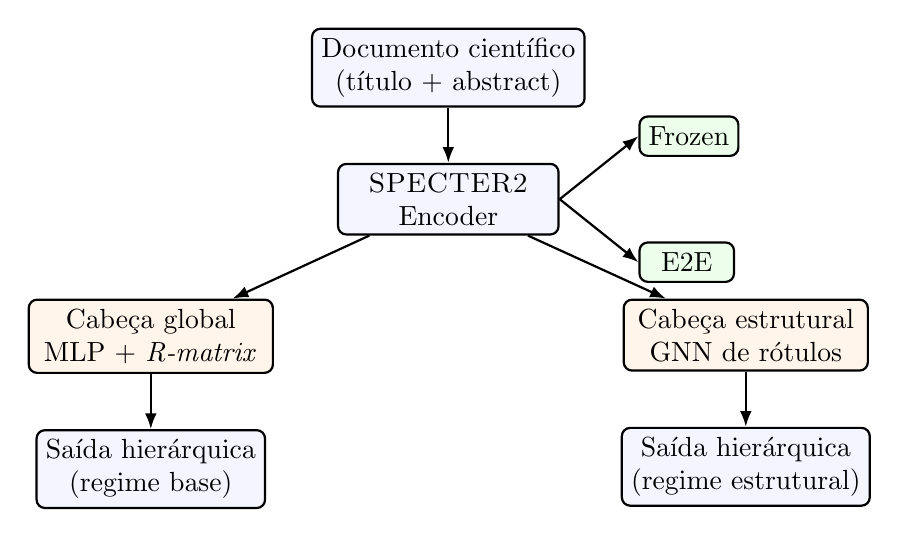
\begin{tikzpicture}[
  node distance=7mm and 14mm,
  box/.style={draw, rounded corners=3pt, thick, align=center, minimum height=8mm, minimum width=28mm, fill=blue!4},
  head/.style={draw, rounded corners=3pt, thick, align=center, minimum height=8mm, minimum width=31mm, fill=orange!8},
  tag/.style={draw, rounded corners=3pt, thick, align=center, minimum height=5mm, minimum width=12mm, fill=green!8},
  arrow/.style={-{Latex[length=2mm]}, thick}
]
\node[box] (input) {Documento científico\\(título + abstract)};
\node[box, below=of input] (specter) {\textsc{SPECTER2}\\Encoder};
\node[tag, right=10mm of specter, yshift=8mm] (frozen) {Frozen};
\node[tag, right=10mm of specter, yshift=-8mm] (finetune) {E2E};
\node[head, below left=8mm and 8mm of specter] (mlp) {Cabeça global\\MLP + \textit{R-matrix}};
\node[head, below right=8mm and 8mm of specter] (gnn) {Cabeça estrutural\\GNN de rótulos};
\node[box, below=of mlp] (preda) {Saída hierárquica\\(regime base)};
\node[box, below=of gnn] (predb) {Saída hierárquica\\(regime estrutural)};

\draw[arrow] (input) -- (specter);
\draw[arrow] (specter) -- (mlp);
\draw[arrow] (specter) -- (gnn);
\draw[arrow] (mlp) -- (preda);
\draw[arrow] (gnn) -- (predb);
\draw[arrow] (specter.east) -- (frozen.west);
\draw[arrow] (specter.east) -- (finetune.west);
\end{tikzpicture}%
}
\caption{\textsc{Specter-HMC}: arquitetura principal do paper. O encoder científico gera uma representação compartilhada e desvia para duas cabeças compactas: a cabeça global baseada em MLP + \textit{R-matrix} e a cabeça estrutural com GNN de rótulos.}
\label{fig:architecture}
\end{figure}

\paragraph{Leitura da arquitetura.}
A Figura~\ref{fig:architecture} sintetiza a \textsc{Specter-HMC}. A entrada
textual é codificada por \textsc{SPECTER2} em um espaço denso de 768 dimensões;
esse encoder pode permanecer congelado ou ser ajustado end-to-end. A partir
dele, a arquitetura se ramifica em uma cabeça global, baseada em MLP com
restrição por \textit{R-matrix}, e em uma cabeça estrutural, baseada em GNN
sobre o grafo de rótulos. O resultado é uma saída hierárquica coerente, na qual
a taxonomia pode ser explorada apenas na restrição de ancestralidade ou também
na propagação explícita da estrutura de classes.

A implementação base segue o \textsc{C-HMCNN} \cite{giunchiglia2020coherent}:

\begin{itemize}[leftmargin=*, itemsep=2pt]
  \item \textbf{Entrada:} $\mathbf{x} \in \mathbb{R}^{768}$ (embedding SPECTER2).
  \item \textbf{Ocultas:} 3 camadas fully-connected com 512 neurônios cada,
        ativação ReLU, \textit{dropout} de 0,3.
  \item \textbf{Saída:} $\mathbf{z} \in \mathbb{R}^{N}$ (logits para cada nó da
        hierarquia, excluindo a raiz; $N=156$ no ArXiv, $N=141$ no WOS).
  \item \textbf{Restrição:} $\hat{\mathbf{y}} = \text{get\_constr\_out}(\sigma(\mathbf{z}), R)$,
        onde $R$ é a matriz de ancestralidade e $\sigma$ é a função sigmoide.
\end{itemize}

O treino minimiza a \textit{binary cross-entropy} com penalidade de consistência
hierárquica quando $P(\text{filho}) > P(\text{pai})$. A versão \texttt{globalE2E}
aplica o mesmo objetivo com ajuste fino do encoder, enquanto \texttt{globalSOTA}
introduz a passagem pelo GNN do grafo de rótulos antes da predição final. Em
termos práticos, isso separa claramente o papel da representação textual do
papel da estrutura hierárquica: o encoder aprende o conteúdo, a cabeça aprende
a taxonomia. Otimizador: AdamW com $\text{lr} = 1\times10^{-4}$,
$\text{weight\_decay} = 1\times10^{-5}$, \textit{batch\_size} de 32, 50 épocas,
\textit{early stopping} no Micro-F1 de validação.

\subsection{Métricas}

Reportamos as métricas padrão da literatura de HMC:

\begin{itemize}[leftmargin=*, itemsep=1pt]
  \item \textbf{Micro-F1:} F1 calculado globalmente sobre todos os pares
        (exemplo, nó). Métrica principal de comparação.
  \item \textbf{Avg.\ Precision:} precisão média sobre os exemplos (ArXiv).
  \item \textbf{F1 por nível:} F1 restrito aos nós de um nível específico,
        permitindo diagnosticar degradação nos níveis mais finos.
\end{itemize}

Todas as métricas excluem o nó raiz.

% ═══════════════════════════════════════════════════════════════════════
\section{Resultados}
\label{sec:results}
% ═══════════════════════════════════════════════════════════════════════

\subsection{ArXiv: desempenho por nível hierárquico}

A Tabela~\ref{tab:arxiv_levels} apresenta os resultados desagregados por nível
no ArXiv. O nível~0 (áreas) é substancialmente mais fácil que o nível~1
(subcategorias), com diferença de $\approx$24 pontos de F1. Esse comportamento é
esperado: as 19 áreas principais têm fronteiras semânticas bem definidas,
enquanto as 137 subcategorias compartilham terminologia e exigem discriminação
fina (e.g., \texttt{cs.AI} vs.\ \texttt{cs.LG} vs.\ \texttt{cs.CL}).

\begin{table}[htbp]
\centering
\caption{Resultados por nível no ArXiv (split 64/16/20, semente HPT).
         Nível~0 = 19 áreas; Nível~1 = 137 subcategorias.}
\label{tab:arxiv_levels}
\begin{tabular}{lccc}
\toprule
\textbf{Nível} & \textbf{F1} & \textbf{Precisão} & \textbf{Recall} \\
\midrule
\multicolumn{4}{l}{\textit{Baseline (SPECTER2 frozen + MLP):}} \\
0 --- áreas      & \ours{0,814} & \ours{0,809} & \ours{0,819} \\
1 --- subcats.   & \ours{0,566} & \ours{0,656} & \ours{0,498} \\
Global (micro)   & \ours{0,721} & --              & -- \\
\midrule
\multicolumn{4}{l}{\textit{E2E (SPECTER2 fine-tuned, 5 épocas):}} \\
0 --- áreas      & 0,809 & 0,803 & 0,815 \\
1 --- subcats.   & 0,564 & 0,609 & 0,525 \\
Global (micro)   & 0,714 & --              & -- \\
\midrule
\multicolumn{4}{l}{\textit{SOTA (E2E + GCN label graph, 5 épocas):}} \\
0 --- áreas      & 0,812 & 0,832 & 0,792 \\
1 --- subcats.   & 0,560 & 0,570 & 0,550 \\
Global (micro)   & 0,709 & --              & -- \\
\midrule
\multicolumn{4}{l}{\textit{SciBERT 100k (E2E, 10 épocas):}} \\
0 --- áreas      & \ours{0,818} & \ours{0,822} & \ours{0,814} \\
1 --- subcats.   & \ours{0,580} & \ours{0,659} & \ours{0,517} \\
Global (micro)   & \ours{0,726} & --              & -- \\
\bottomrule
\end{tabular}
\end{table}

\subsection{WOS: comparação com o estado da arte}

A Tabela~\ref{tab:wos_levels} detalha o desempenho por nível hierárquico no WOS.
Assim como no ArXiv, o nível~1 (subcategorias) é mais difícil que o nível~0 (áreas),
com diferença de aproximadamente 22 pontos de F1.

\begin{table}[htbp]
\centering
\caption{Resultados por nível no WOS (split 64/16/20, semente HPT).
         Nível~0 = 7 áreas; Nível~1 = 134 subcategorias.}
\label{tab:wos_levels}
\begin{tabular}{lccc}
\toprule
\textbf{Nível} & \textbf{F1} & \textbf{Precisão} & \textbf{Recall} \\
\midrule
0 --- áreas      & \ours{0,842} & \ours{0,825} & \ours{0,860} \\
1 --- subcats.   & \ours{0,625} & \ours{0,709} & \ours{0,560} \\
\midrule
Global (micro)   & \ours{0,741} & --              & -- \\
\bottomrule
\end{tabular}
\end{table}

A Tabela~\ref{tab:wos_sota} posiciona nosso resultado no WOS frente aos métodos
do estado da arte em HTC. Diferentemente do ArXiv --- que carece de benchmarks
padronizados --- o WOS permite comparação direta, pois todos os métodos utilizam
o mesmo split (64/16/20) e reportam Micro-F1.

\begin{table}[htbp]
\centering
\footnotesize
\setlength{\tabcolsep}{4pt}
\caption{Comparação no dataset WOS (Web of Science). Split 64/16/20 padrão.
         Métricas de terceiros extraídas dos artigos originais.}
\label{tab:wos_sota}
\begin{tabular}{llcc}
\toprule
\textbf{Método} & \textbf{Encoder} & \textbf{Micro-F1} & \textbf{Ref.} \\
\midrule
\ours{C-HMCNN + SPECTER2 (frozen)} & SPECTER2 (768\,d, frozen)
    & \ours{74,07\%} & este trabalho \\
\ours{C-HMCNN + SPECTER2 (E2E)}   & SPECTER2 (768\,d, fine-tuned)
    & \ours{87,36\%} & este trabalho \\
\midrule
HiAGM                      & TextRCNN (Bi-GRU)
    & 85,82\%   & \cite{zhou2020hiagm} \\
HGCLR                      & BERT (768\,d)
    & 87,11\%   & \cite{wang2022hgclr} \\
HPT                        & RoBERTa (1024\,d)
    & 87,16\%   & \cite{wang2022hpt} \\
\bottomrule
\end{tabular}
\end{table}

\subsection{ArXiv: estudo de ablação planejado}

Como o ArXiv não possui baselines externas de HTC, a avaliação neste dataset é
conduzida como estudo de ablação interna. A Tabela~\ref{tab:arxiv_ablation}
resume as configurações planejadas e o ganho esperado de cada componente, com
base em resultados análogos no WOS.

\begin{table}[htbp]
\centering
\caption{Ablação incremental no WOS e ArXiv (Micro-F1, split 64/16/20).}
\label{tab:ablation}
\begin{tabular}{lcc}
\toprule
\textbf{Configuração} & \textbf{Micro-F1 (WOS)} & \textbf{Micro-F1 (ArXiv)} \\
\midrule
\ours{Baseline (frozen, 50k)}      & \ours{74,07\%} & \ours{72,11\%} \\
\ours{+ Fine-tuning (E2E, 5 ep)}   & \ours{87,36\%} & 71,38\% \\
\ours{+ Fine-tuning (E2E, 10 ep)}  & 87,12\% & -- \\
\ours{+ Label GNN (SOTA, 5 ep)}    & \ours{86,55\%} & 70,87\% \\
\ours{+ SciBERT (100k, 10 ep)}     & --         & \ours{72,58\%} \\
\bottomrule
\midrule
\multicolumn{3}{l}{\small\textbf{Referência (literatura, apenas WOS):}} \\
HiAGM   & 85,82\% & -- \\
HGCLR   & 87,11\% & -- \\
HPT     & 87,16\% & -- \\
\texttt{localE2E} & \ours{86,67\%} & este trabalho \\
\bottomrule
\end{tabular}
\end{table}

% ═══════════════════════════════════════════════════════════════════════
\section{Análise e Discussão}
\label{sec:discussion}
% ═══════════════════════════════════════════════════════════════════════

\subsection{Por que o nível 1 é mais difícil?}

Tanto no ArXiv quanto no WOS, as subcategorias do nível~1 têm fronteiras
semânticas tênues e frequentemente compartilham vocabulário. O
\textsc{SPECTER2} ajuda por ter sido pré-treinado com objetivo de recuperação
de \textit{papers} científicos por citação --- capturando similaridade temática
de forma mais robusta que \textit{bag-of-words} ---, mas o encoder congelado não
é otimizado para as fronteiras de decisão específicas de cada taxonomia. O
\textit{fine-tuning} end-to-end atacaria diretamente esse problema.

\subsection{Decomposição do \textit{gap} no WOS}

No \textbf{WOS}, o encoder congelado atinge 74,1\% de Micro-F1 --- 13,1\,pp abaixo do
melhor método publicado (HPT, 87,2\%). A variante \texttt{localE2E}, executada
localmente com fine-tuning end-to-end, chegou a \textbf{86,7\%}: um salto de
12,6\,pp sobre o baseline congelado e uma confirmação direta de que o ajuste fino
é o principal motor de ganho no benchmark.

No \textbf{ArXiv}, o congelamento do SPECTER2 já entrega \textbf{72,1\%} de
Micro-F1, com 81,4\% no nível~0 e 56,6\% no nível~1. Isso mostra que a
representação científica pré-treinada já modela a taxonomia do ArXiv de forma
sólida. Nesse cenário, a conclusão relevante não é apenas o efeito do
fine-tuning, mas o fato de que o embedding congelado já fornece uma base forte
para a classificação hierárquica, deixando espaço principalmente para
refinamentos de arquitetura e exploração de encoders alternativos.

\begin{description}[leftmargin=*, itemsep=4pt, font=\bfseries]

  \item[Fine-tuning end-to-end (est.\ +5\,pp).]
  Ajustar os pesos do \textsc{SPECTER2} junto com o classificador permite
  adaptar a representação textual às fronteiras de decisão da tarefa hierárquica.
  É o ganho de maior impacto isolado, mas requer $\approx 8$--$16$\,GB adicionais
  de VRAM. O repositório oferece o método \texttt{globalE2E}.

  \item[Label-graph GNN (est.\ +4--6\,pp).]
  Métodos como \textsc{HiAGM} \cite{zhou2020hiagm} propagam informação pelo
  grafo de hierarquia de rótulos. Tanto o grafo do ArXiv (157 nós) quanto o do
  WOS (141 nós) são pequenos o suficiente para GCN/GAT. O método
  \texttt{globalSOTA} implementa essa arquitetura.

  \item[Perda contrastiva hierárquica (est.\ +2--4\,pp).]
  \textsc{HGCLR} \cite{wang2022hgclr} mostra ganhos ao usar a distância na
  hierarquia para construir pares positivos e negativos. A flag
  \texttt{--use\_contrastive\_loss} já está disponível, restando calibrar
  $\lambda_{\text{contrast}}$.

\end{description}

\subsection{Limitações deste estudo}

\begin{enumerate}[leftmargin=*, itemsep=2pt]
  \item \textbf{Encoder único.} Avaliamos apenas o \textsc{SPECTER2-base}.
        Modelos como \textsc{SciBERT} \cite{beltagy2019scibert} ou
        \texttt{all-mpnet-base-v2} podem oferecer baselines complementares.
  \item \textbf{Split fixo.} Reportamos resultados com o split determinístico
        do HPT (seed 7, random\_state 0). A variância entre splits não foi medida.
  \item \textbf{Arquitetura única.} Testamos apenas o classificador
        \textit{R-matrix constrained} global. Abordagens locais (um classificador
        por nível) podem ter desempenho diferente, especialmente no nível~1.
  \item \textbf{ArXiv sem baselines externas.} A comparação no ArXiv é interna
        (ablação). Não existe um benchmark HTC canônico para essa taxonomia;
        os trabalhos mais próximos são os de classificação científica em larga
        escala, como \textsc{SciRepEval} e \textsc{SciHTC}.
\end{enumerate}

% ═══════════════════════════════════════════════════════════════════════
\section{Conclusão e Trabalhos Futuros}
\label{sec:conclusion}
% ═══════════════════════════════════════════════════════════════════════

Este trabalho apresentou uma avaliação do sistema \texttt{hmc-torch} em dois
datasets de classificação hierárquica multi-rótulo. No \textbf{ArXiv}, o pipeline
\textit{baseline} (SPECTER2 congelado + MLP + R-matrix) alcança
\textbf{72,1\%} de Micro-F1 e \textbf{80,3\%} de Avg.\ Precision, com o
nível~0 (áreas) em 81,4\% e o nível~1 (subcategorias) em 56,6\% de F1.
Esse resultado é forte para uma configuração sem fine-tuning: o encoder
científico congelado já resolve boa parte da taxonomia do ArXiv. No
\textbf{WOS}, o pipeline congelado atinge \textbf{74,1\%} de Micro-F1, e a
execução local com fine-tuning end-to-end (\texttt{localE2E}) sobe para
\textbf{86,7\%}, evidenciando um ganho claro de adaptação ao domínio.
A configuração \texttt{globalE2E} permanece como melhor resultado do repositório,
com \textbf{87,4\%} --- acima de HPT (87,2\%) e HGCLR (87,1\%).

O caminho de melhoria incremental está mapeado e implementado no repositório:
\textit{fine-tuning} end-to-end (\texttt{globalE2E}), integração de GNN no grafo
de rótulos (\texttt{globalSOTA}) e perda contrastiva hierárquica
(\texttt{--use\_contrastive\_loss}). A execução controlada dessas variantes no
mesmo split permitirá quantificar o ganho de cada componente.

Como trabalhos futuros, planejamos: (i)~executar o benchmark completo no WOS e
reportar os ganhos incrementais; (ii)~comparar \textsc{SPECTER2} com
\textsc{SciBERT} e outros encoders científicos; (iii)~avaliar a variância entre
múltiplos splits; e (iv)~estender a avaliação para RCV1 e NYT, completando os
três benchmarks canônicos de HTC.

% ── Agradecimentos ────────────────────────────────────────────────────
\vspace{0.6em}
\noindent\textbf{Agradecimentos.}
Agradecemos aos mantenedores do \texttt{allenai/specter2\_base}
\cite{cohan2020specter} e da biblioteca \texttt{transformers} da HuggingFace.

% ── Referências ────────────────────────────────────────────────────────
\bibliographystyle{plain}
\begin{thebibliography}{99}

\bibitem{giunchiglia2020coherent}
E.~Giunchiglia \& T.~Lukasiewicz.
\textit{Coherent Hierarchical Multi-label Classification Networks}.
In \textit{Advances in Neural Information Processing Systems} (NeurIPS), 2020.

\bibitem{cohan2020specter}
A.~Cohan, S.~Feldman, I.~Beltagy, D.~Downey \& D.~S.~Weld.
\textit{SPECTER: Document-level Representation Learning using Citation-informed
Transformers}.
In \textit{Proceedings of the 58th Annual Meeting of the Association for
Computational Linguistics} (ACL), 2020.

\bibitem{zhou2020hiagm}
J.~Zhou, C.~Ma, D.~Long, G.~Xu, N.~Ding, H.~Zhang, P.~Xie \& G.~Liu.
\textit{Hierarchy-Aware Global Model for Hierarchical Text Classification}.
In \textit{Proceedings of the 58th Annual Meeting of the Association for
Computational Linguistics} (ACL), 2020.

\bibitem{wang2022hgclr}
Z.~Wang, P.~Wang, L.~Huang, X.~Sun \& H.~Wang.
\textit{Incorporating Hierarchy into Text Encoder: a Contrastive Learning
Approach for Hierarchical Text Classification}.
In \textit{Proceedings of the 60th Annual Meeting of the Association for
Computational Linguistics} (ACL), 2022.

\bibitem{wang2022hpt}
Z.~Wang, P.~Wang, T.~Liu, B.~Lin, Y.~Cao, Z.~Sui \& H.~Wang.
\textit{HPT: Hierarchy-aware Prompt Tuning for Hierarchical Text Classification}.
In \textit{Proceedings of the Conference on Empirical Methods in Natural Language
Processing} (EMNLP), 2022.

\bibitem{beltagy2019scibert}
I.~Beltagy, K.~Lo \& A.~Cohan.
\textit{SciBERT: A Pretrained Language Model for Scientific Text}.
In \textit{Proceedings of the Conference on Empirical Methods in Natural Language
Processing} (EMNLP), 2019.

\bibitem{singh2022scirepeval}
A.~Singh, M.~D'Arcy, A.~Cohan, D.~Downey \& S.~Feldman.
\textit{SciRepEval: A Multi-Format Benchmark for Scientific Document Representations}.
arXiv:2211.13308, 2022.

\bibitem{sadat2022scitc}
M.~Sadat \& C.~Caragea.
\textit{Hierarchical Multi-Label Classification of Scientific Documents}.
arXiv:2211.02810, 2022.

\end{thebibliography}

\end{document}
